% Created 2017-01-17 Tue 11:30
% Intended LaTeX compiler: pdflatex
\documentclass[aps,prl,reprint,groupedaddress,amsmath,amssymb, showpacs]{revtex4-1}
 \usepackage{minted}
 \usepackage{graphicx}
\usepackage{float}
\usepackage{xcolor}
\usepackage{fontspec}
\date{}
\title{}
\begin{document}

\title{A Multiscale View of the Doping-Induced Tunable Wettability on Two-Dimensional Materials}
\author{Tian Tian} 
  \affiliation{Institute for Chemical and Bioengineering, ETH Z{\"{u}}rich,  Vladimir Prelog Weg 1, CH-8093 Z{\"{u}}rich, Switzerland}
\author{Elton J. G. Santos}
  \affiliation{School of Mathematics and Physics, Queen's University Belfast, United Kingdom}
  \affiliation{School of Chemistry and Chemical Engineering, Queen's University Belfast, United Kingdom}
\author{Shangchao Lin}
  \email{slin@eng.fsu.edu.}
  \affiliation{Department of Mechanical Engineering, Materials Science and Engineering Program, FAMU-FSU College of Engineering, Florida State University, Tallahassee, Florida 32310, United States}
\author{Chih-Jen Shih}
  \email{chih-jen.shih@chem.ethz.ch}
  \affiliation{Institute for Chemical and Bioengineering, ETH Z{\"{u}}rich,  Vladimir Prelog Weg 1, CH-8093 Z{\"{u}}rich, Switzerland}

\date{\today}

\begin{abstract}
  The emergence of 2D-material-based liquid-phase devices calls for
  the need for understanding the wetting property at the
  2D-material-liquid interface, and particularly the doping-induced
  tuning of wetting properties. In this letter, we propose a
  multiscale view of the doping-induced tunable wettability of 2D
  materials, by combining the reorientation effect of water molecules
  estimated by MD simulation, and the electrowetting effect calculated
  by continuum model. We reveal the electrostatic nature of the
  doping-induced wettability under both scale. We further evaluate the
  recent finding of doping-induced wettability tuning of graphene with
  the proposed model, by considering incomplete surface coverage of 2D
  materials. We find that minor surface incompleteness can cause great
  discrepancy in the measured value of interfacial wettability, requiring
  extreme care for interpreting the experimental results. In
  addition, we prove that a 2D material with higher density of states
  can essentially reduce the gating voltage in a 2D-material-based
  electrowetting device, and rank the tunability of the 2D materials
  as: MoTe$_{2}$ > MoS$_{2}$ > WTe$_{2}$ > WS$_{2}$ > germanene > silicene >
  graphene. Our multiscale analysis provides a comprehensive view of
  the wettability of 2D material interface, and we believe operational
  2D-material-based liquid manipulating devices will be facilitate by
  the principles presented in this letter.
\end{abstract}
\maketitle

The emergence of two-dimensional (2D) materials has attracted broad
interest in various research fields, inspired by their unique physical
and chemical properties. Recent progress of scalable 2D material
synthesis paves the way for their liquid phase 2D-material-based
applications, for instance functional coating
\cite{Prasai_2012,Rafiee_2010,Kim_2014}, nanotribology devices
\cite{Yin_2014,Tang_2016,Feng_2016}, nanoporous desalination apparatus
\cite{Surwade_2015,Rollings_2016,Jain_2015}, droplet manipulation
\cite{Hern_ndez_2013,Vijayarangamuthu_2015}, etc.  To fully exploit the
physics of the interface between 2D materials and liquid phase, a
comprehensive understanding of the 2D-material-liquid interaction, and in
particular, the wettability, is of great importance.


Wetting on atomically-thin 2D materials has long been a hot but highly
disputed topic
\cite{taherian2013what,Kozbial_2015,Parobek_2015,Govind_Rajan_2016}.
Accurate description of the intrinsic wettability of 2D materials is
known to be challenging. Recent studies show that the wettability on
graphene \cite{li_effect_2013,Xu_2013_withwhat,kozbial_study_2014} and
MoS\(_{\text{2}}\) \cite{Kozbial_2015,Chow_2015} is strongly affected by airborne
contaminants. Meanwhile, the contact angle measurement technique which
has been widely to determine the wettability on 2D materials, may also
suffer inaccuracy from contact angle hysteresis caused by local
defects \cite{raj_wettability_2013}.  On the other hand, unlike bulk
materials, the thickness of a 2D material falls within the effective
range of dispersion interactions.  As a result, the dispersion
interaction between the substrate underneath the 2D material and
liquid molecules is not fully screened by the 2D material, giving rise
to the fascinating property known as the ``wetting-translucency''
\cite{rafiee_wetting_2012,shih_breakdown_2012,shih_wetting_2013}.
Moreover, 2D semimetals (graphene, silecene, germanene, etc.) and 2D
semiconductors (e.g, transition metal dichalcogenides (TMDCs)) possess
significantly lower density of states (DOS) than bulk materials,
making them easier to be doped by the underlying substrates
\cite{Chen_2013,Varchon_2007,Giovannetti_2008} or electrostatic gating
\cite{Das_2008,Perera_2013}. Due to the ubiquity of doping in 2D
materials, it is worth investigating the relationship between the
doping level and wettability. Several recent reports have addressed
the issue of doping-induced tunability of graphene's wettability, from
both atomistic simulations
\cite{ostrowski_tunable_2014,ren_interfacial_2015,Taherian_2015,daub_electrowetting_2007}
and experimental demonstrations
\cite{hong_mechanism_2016,goniszewski_correlation_2016,ashraf_doping-induced_2016}.
However, discrepancies exist between individual reports, concerning
the origin and magnitude of the doping-induced wetting
tunability. Moreover, to get a full perspective of such phenomenon,
the gap between the nanoscale simulations and macroscopic experimental
results needs to be filled, and the aforementioned issues of intrinsic
wettability and wetting translucency should also be taken into account.

In this letter, we propose a multiscale approach to properly model the
doping-induced tuning of 2D materials' wettability. We model the
change of surface adhesion energy between water and 2D material as a
combined effect of (i) reorientation of water molecules, characterized
by molecular dynamic (MD) simulations and (ii) electrowetting due to
formation of electric double layer, calculated by a continuum model
based on modified Young-Lippman theory. By using graphene as an
example, we demonstrate that, the electrostatic interaction plays a
major role in both the reorientation and electrowetting effects. By
further considering the surface coverage of 2D materials, we evaluate
the previous reported result on the doping-induced wetting behavior of
graphene using the proposed multiscale model. We find that the
existence of minor defects can cause great discrepancy between the
observed wetting property and theoretical values, requesting attentive
interpretation of the experimental results. Moreover, we quantify the
tunability of interfacial tension in a gate-controlled
2D-material-based electrowetting device as a function of the DOS of
the 2D material, and rank several 2D materials according to their
tunability. We show that 2D materials with higher DOS such as
transition metal dichalcogenides (TMDCs), perform better than graphene
by means of wettability regulation. Our findings provide a
comprehensional view of the wettability of 2D materials, as well as
guidance for operational liquid-phase 2D material-based devices.



Due to the complex dynamic nature of wetting
\cite{Cassie_1944,Wenzel_1936,Gao_2007,Marmur_2009}, we only study the
static wettability of 2D materials. We only consider water as the
liquid phase, as most liquid-phase applications of 2D materials are
also in aqueous environment. The macroscopic feature of
wetting--contact angle \(\theta\), is connected to the interfacial
adhesion energy \(\Phi_{\mathrm{2D-w}}\) by the Young's equation:
\begin{equation}
\label{eqn:young's equation}
\Phi_{\mathrm{2D-w}} = -\gamma_{\mathrm{L}}(1+\cos\theta)
\end{equation}
where \(\Phi_{\mathrm{2D-w}}\) is defined as:
\begin{equation}
\label{eqn:def-adhesion}
\Phi_{\mathrm{2D-w}} = \gamma_{\mathrm{2D-w}} - \gamma_{\mathrm{2D}} - \gamma_{\mathrm{w}}
\end{equation}

where \(\gamma_{\mathrm{2D-w}}\) is the surface tension between the
interface of the 2D material and the aqueous phase,
\(\gamma_{\mathrm{2D}}\) and \(\gamma_{\mathrm{w}}\) are the surface
tensions of the 2D material and water in vacuum,
respectively. \(\Phi_{\mathrm{2D-w}}\) is contributed by both the
short-range dispersion interaction and long-range electrostatic
interaction between the 2D material and water. The existence of
additional charges in 2D materials gives rise to the reorientation of
adjacent water molecules \cite{ostrowski_tunable_2014}. On the other
hand, the formation of electric double layer (EDL) in an ionic
solution near the interface also alters the interfacial adhesion
properties, known as the electrowetting effect \cite{Lippmann_1908},
which has been widely used in microfluidic applications
\cite{Mugele_2005}.  Owing to the additive nature of dispersion and
electrostatic interactions, we propose that the change of interfacial
adhesion energy \(\Delta \Phi_{\mathrm{2D-w}}\) is a combined effect of
the reorientation effect \(\Delta \Phi_{\mathrm{2D-w}}^{\mathrm{or}}\) and EDL
formation \(\Delta \Phi_{\mathrm{2D-w}}^{\mathrm{el}}\):
\begin{equation}
\label{eqn:contrib-adhesion-change}
\Delta \Phi_{\mathrm{2D-w}} = \Delta \Phi_{\mathrm{2D-w}}^{\mathrm{or}}
                              + \Delta \Phi_{\mathrm{2D-w}}^{\mathrm{el}}
\end{equation}

A multiscale approach is needed to combine both effects as their
effective length scales are different. We use molecular dynamics (MD)
simulations for sampling the orientation effect adjacent to the 2D
material; in addition a continuum model is implemented to describe the
contribution of EDL formation, since state-of-art MD simulations fail to
handle diluted ionic solution systems where the Debye length can be as
long as 10\(^{\text{3}}\) nm. Our multiscale modeling approach is schematically illustrated in Fig. \ref{fig:scheme-method}.

\begin{figure}[htbp]
\centering
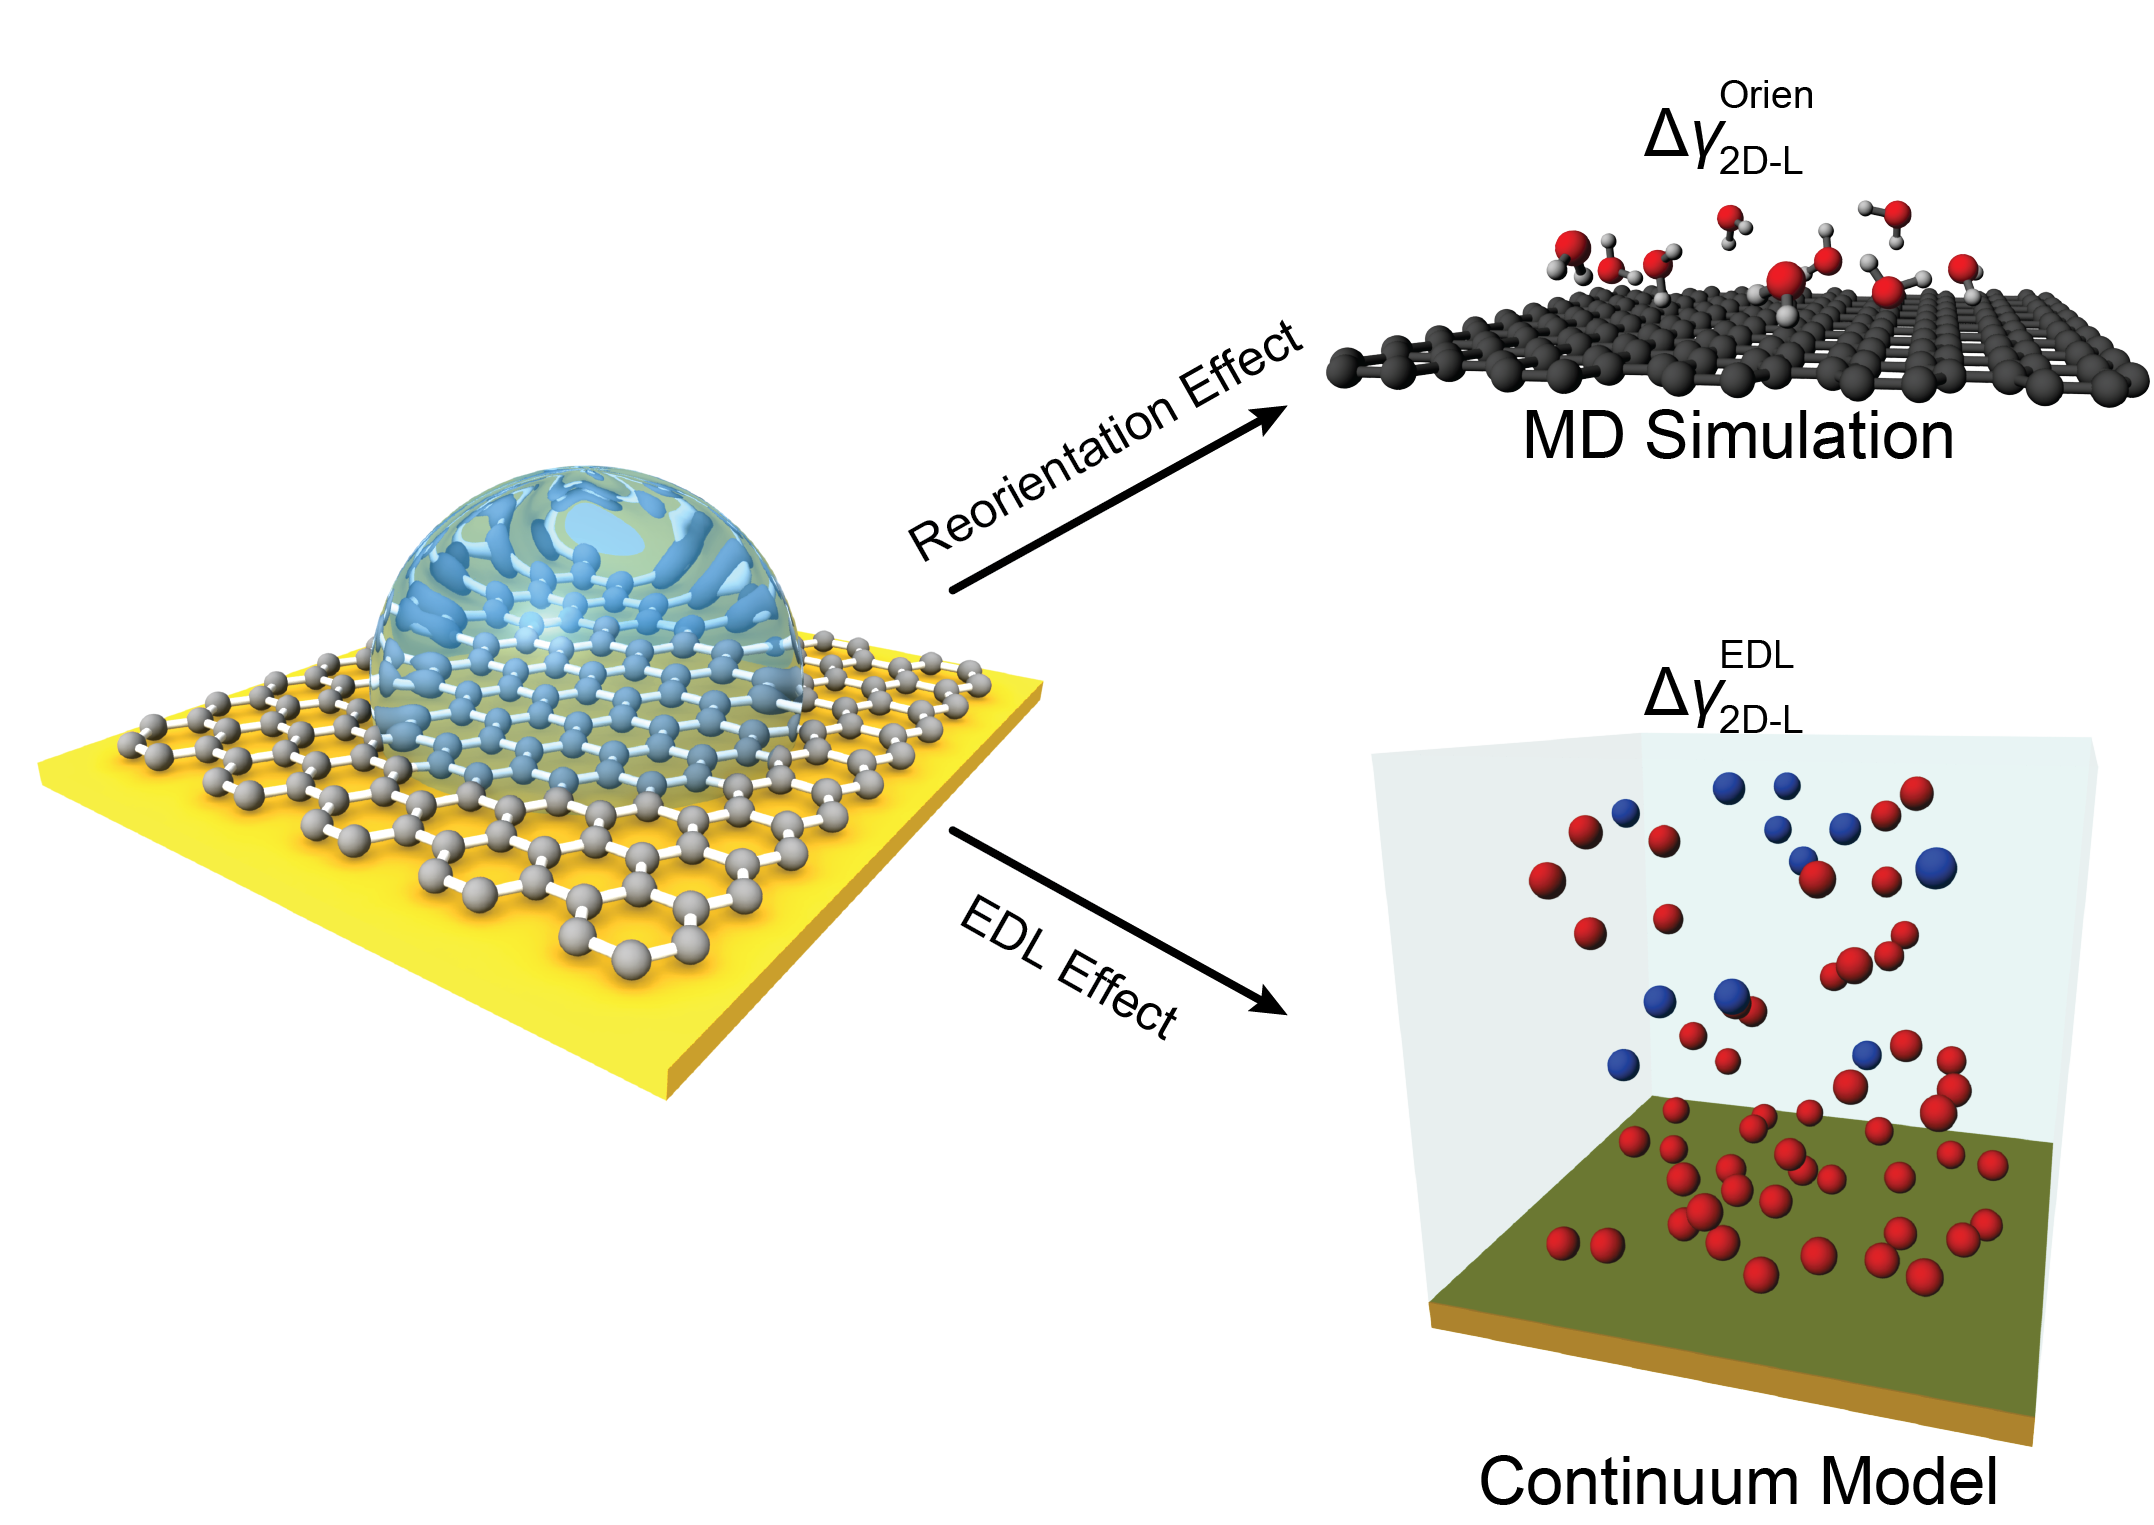
\includegraphics[width=0.95\linewidth]{../img/scheme-methods.pdf}
\caption{\label{fig:scheme-method}
Scheme of the multiscale approach for modeling the doping-induced wettability tuning of 2D materials.}
\end{figure}

It is also noteworthy that our multiscale approach is compatible with
the issues of the intrinsic wettability and wetting translucency of 2D
materials. Since we are dealing with the change of interfacial
adhesion energy as a function of surface charge, the absolute value of
\(\Phi_{\mathrm{2D-w}}\) or \(\gamma_{\mathrm{2D-w}}\) (extracted from intrinsic wetting property and wetting translucency theory) can be treated as
independent variables.


We model the charged 2D materials as rigid sheets with uniform surface
charge density \(\sigma_{\mathrm{2D}}\), either by substrate or
electrostatic doping. We also assume that the 2D material has no
dissociable groups which can change the aqueous pH value
\cite{zuccaro_tuning_2015} and the 2D material is inert to
electrochemical reaction at the interface
\cite{bard_electrochemical_1980}.  First we use graphene as a model
system to show the effect of reorientation of water molecules on the
interfacial adhesion energy. Different from previous approaches which
used MD simulations to extract the contact angle of nanodroplets on
graphene
\cite{ostrowski_tunable_2014,daub_electrowetting_2007,ren_interfacial_2015,Taherian_2015},
where the interfacial adhesion energy cannot be accurately measured
due to changed contact area between water and graphene, here we
propose to use a continuous water monolith in the MD simulation with periodic boundary conditions in the x and y directions to
calculate the interfacial adhesion energy \(\Phi_{\mathrm{2D-w}}\).
\begin{center}
\fbox{
\begin{minipage}[c]{.8\linewidth}
\textbf{\textsf{\textsc{TODO}}} Description for MD simulation

\end{minipage}
}
\end{center}


The adhesion energy \(\Phi_{\mathrm{2D-w}}^{or}\) in the MD simulation is
defined as:
\begin{equation}
\label{eqn:Delta-Phi-or-definition}
\begin{aligned}
\Phi_{\mathrm{2D-w}}^{or} &= (\Psi_{\mathrm{2D-w}} - \Psi_{\mathrm{w}} - \Psi_{\mathrm{2D}})\frac{1}{S \cdot N_{\mathrm{A}}} \\
                     &= \Phi_{\mathrm{LJ}} + \Phi_{\mathrm{CL}}
\end{aligned}
\end{equation}
where \(S\) is the area of the graphene sheet (same as the contact area
 between water and graphene), \(N_{\mathrm{A}}\) is the Avogadro's
 number, \(\Psi_{\mathrm{2D-w}}\) is the total internal potential of the
 2D material-water system, and \(\Psi_{\mathrm{w}}\) and
 \(\Psi_{\mathrm{2D}}\) are the potentials of the separated water phase
 and 2D materials, respectively.  The adhesion energy can be further
 decomposed into the short-range Lenard-Jones potential term
 (\(\Phi_{\mathrm{LJ}}\)) and the long-range Coulombic interaction term
 (\(\Phi_{\mathrm{CL}}\)). Since \(\Psi_{\mathrm{w}}\) and
 \(\Psi_{\mathrm{2D}}\) are unalterable in the MD simulation, the change
 of interfacial adhesion energy \(\Delta \Phi_{\mathrm{2D-w}}^{or}\) as a
 result of surface doping, is calculated as:
\begin{equation}
\label{eqn:delta-Phi-2D-or}
\begin{aligned}
\Delta \Phi_{\mathrm{2D}}^{or} &= \frac{\Delta \Phi_{\mathrm{2D-w}}}{S \cdot N_{\mathrm{A}}} \\
                               &= \Delta \Phi_{\mathrm{LJ}} + \Delta \Phi_{\mathrm{CL}}
\end{aligned}
\end{equation}
\begin{figure}[htbp]
\centering
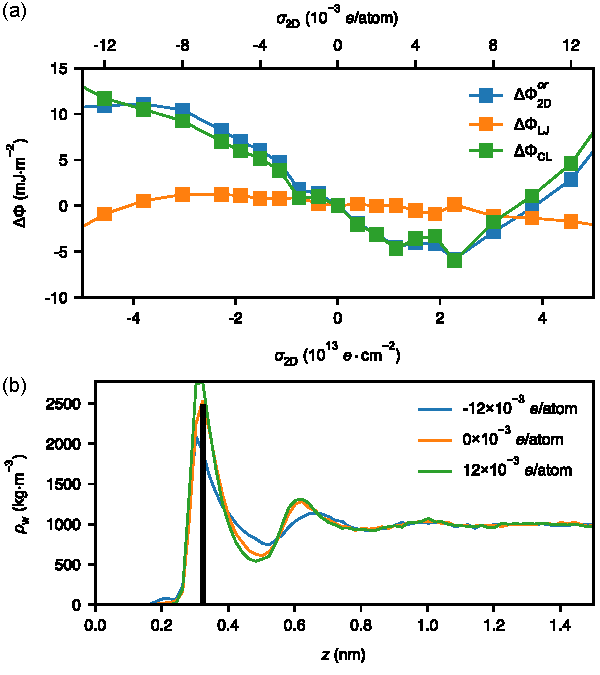
\includegraphics[width=0.9\linewidth]{../img/fig-pot-dens.pdf}
\caption{\label{fig:pot-dens}
(a) Change of total adhesion energy \(\Delta\Phi_{\mathrm{2D}}^{or}\), contribution of Lenard-Jones interaction \(\Delta\Phi_{\mathrm{LJ}}\) and Coulombic interaction \(\Delta\Phi_{\mathrm{CL}}\), as a function of charge density on graphene. (b) Local density of water molecule (\(\rho_{\mathrm{w}}\))  as a function of distance \(z\) from graphene surface.}
\end{figure}


The changes of adhesion energy terms \(\Delta
\Phi_{\mathrm{2D-w}}^{or}\), \(\Delta \Phi_{\mathrm{LJ}}\) and \(\Delta
\Phi_{\mathrm{CL}}\), as functions of \(\sigma_{\mathrm{2D}}\) , are
shown in Fig. \ref{fig:pot-dens}(a). It can be seen that the
contribution from dispersion interaction \(\Delta \Phi_{\mathrm{LJ}}\)
has a very small magnitude of negative change (less than 2.5 mJ\(\cdot
\mathrm{m}^{-2}\)) when \(\sigma_{\mathrm{2D}}\) ranges from
-5\(\times10^{13}\) \textasciitilde{} 5\(\times10^{13}\) \(e\cdot \mathrm{cm}^{-2}\). On the
other hand, we find that \(\Delta \Phi_{\mathrm{CL}}\) contributes
majorly to \(\Delta \Phi_{\mathrm{2D-w}}^{or}\), indicating the
electrostatic nature of the doping-induced reorientation of water
molecules.
\begin{center}
\fbox{
\begin{minipage}[c]{.8\linewidth}
\textbf{\textsf{\textsc{TODO}}} Validate the statement above

\end{minipage}
}
\end{center}
It is also interesting to find that, unlike its counterpart from
dispersion interaction, \(\Delta \Phi_{\mathrm{CL}}\) has a asymmetric
response to \(\sigma_{\mathrm{2D}}\). We further plot the local density
of water molecules \(\rho_{\mathrm{w}}\), as a function of distance \(z\)
from the graphene plane, which can be seen in Fig. \ref{fig:pot-dens}(b). We consider
3 cases where the graphene layer is either charge-neutral, or
\(\sigma_{\mathrm{2D}}=\pm 0.012\ e/ \mathrm{atom}\), respectively. We
find that the \(\rho_{\mathrm{w}}\) at the first water layer adjacent to
graphene (\(z \approx 3.2\ \mathrm{\AA}\)) also responsed asymmetrically with
\(\sigma_{\mathrm{2D}}\).  When \(\sigma_{\mathrm{2D}}=-0.012\ e/
\mathrm{atom}\), \(\rho_{\mathrm{w}}\) drops to ca. 80\% of that in the
electroneutral system, while \(\rho_{\mathrm{w}}\) at
\(\sigma_{\mathrm{2D}}=0.012\ e/ \mathrm{atom}\) has a 8\% increase in the density compared with the electroneutral system. The change of interfacial water
density can be ascribed by the polarity of water molecules. When the
graphene layer is positively charged, the O atom is more favorably
facing the graphene surface, while H atom is more favorably facing the
negatively-charged surface.
\begin{center}
\fbox{
\begin{minipage}[c]{.8\linewidth}
\textbf{\textsf{\textsc{TODO}}} Describe the density change

\end{minipage}
}
\end{center}
\begin{center}
\fbox{
\begin{minipage}[c]{.8\linewidth}
\textbf{\textsf{\textsc{TODO}}} More in-depth discussion?

\end{minipage}
}
\end{center}

It is noteworthy that although the process for investigating the
magnitude of \(\Delta \Phi_{\mathrm{2D-w}}^{or}\) is similar for other 2D
materials other than graphene, the result obtained here cannot be
readily applied to other 2D materials, since the contribution of
dispersion interaction and electrostatic interaction can be completely
different \cite{Govind_Rajan_2016,Chow_2015}. Nevertheless, in
real-world measurements, due to the existence of the contamination
layer which has a typical thickness ca. 1\textasciitilde{}2 nm, the dispersion
interactions contributed by surface charge can be nearly completely
screened out; aqueous electrolytes can also greatly attenuate the
electric displacement field, compared with the dipole water model used
in the MD simulations. Therefore we propose that the effect of
reorientation may not be easily observable in current experimental
setups.


While the interfacial dispersion interaction vanishes several
molecules away from the surface, the long range electrostatic
interaction will cause the aqueous ions to rearrange at a much longer
length scale, forming an EDL at the interface and decrease the
interfacial surface tension by the phenomenon known as
electrowetting. To model the effect of electrowetting, we first
consider that a contamination layer with thickness \(d_{\mathrm{c}}\)
covers the 2D material surface. Since the airborne contaminants are
mostly hydrocarbon compounds, they can be treated as a dielectric
layer with permittivity \(\epsilon_{\mathrm{c}}\). We use the
Gouy-Chapman-Stern model to describe the EDL in the aqueous phase,
which consists a Helmholtz double layer with the same permittivity
\(\epsilon_{\mathrm{w}}\) as water, and thickness \(d_{\mathrm{H}}\),
together with a diffuse layer where ionic distribution is described by
the Gouy-Chapman equation.  The potentials at the surface of the 2D
material, the contamination layer surface and the outer Helmholtz
plane (the interface between the Helmholtz double layer and the
diffuse layer) are \(\psi_{\mathrm{2D}}^{*}\), \(\psi_{\mathrm{2D}}\) and
\(\psi_{\mathrm{L}}\), respectively. An illustration of the model for the
2D-material-water interface is shown in Fig. \ref{fig:scheme-EDL}.

\begin{figure}[htbp]
\centering
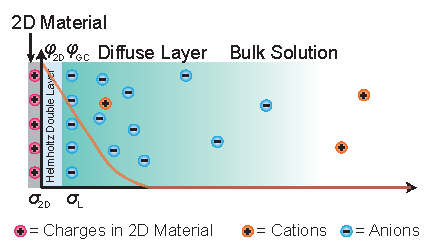
\includegraphics[width=0.95\linewidth]{../img/scheme-EDL.pdf}
\caption{\label{fig:scheme-EDL}
Scheme of the interface between the 2D material and the aqueous phase. A electrostatic potential \(\psi_{\mathrm{2D}}\) is built at the interface, as a result of surface charge on 2D material \(\sigma_{\mathrm{2D}}\).}
\end{figure}

If we neglect specific adsorption of ions at the solid-liquid interface,
electroneutrality ensures that the charge density of the 2D material
\(\sigma_{\mathrm{2D}}\) balances the total charge density of the EDL
\(\sigma_{\mathrm{L}}\) \cite{bard_electrochemical_1980}:
\begin{equation}
\sigma_{\mathrm{2D}} + \sigma_{\mathrm{L}} = 0
\end{equation}
From the Gouy-Chapman model of symmetric electrolytes we know:
\begin{align}
\displaystyle
\label{eqn:psi-L}
\psi_{\mathrm{L}} &= -\frac{2k_{\mathrm{B}}T}{z_{0}e} 
                       \sinh^{-1}\left(
                         \frac{\sigma_{\mathrm{L}}}{\sqrt{8c_{0}N_{\mathrm{A}}\epsilon_{\mathrm{w}}k_{\mathrm{B}}T}}
                          \right) \\
\label{eqn:psi-2D}
\psi_{\mathrm{2D}} &= \psi_{\mathrm{L}} - \sigma_{\mathrm{L}}\frac{d_{\mathrm{H}}}{\epsilon_{\mathrm{w}}} \\
\psi_{\mathrm{2D}}^{*} &= \psi_{\mathrm{2D}} - \sigma_{\mathrm{L}}\frac{d_{\mathrm{c}}}{\epsilon_{\mathrm{c}}}
\end{align} 
where \(z_{0}\) is the valency of the electrolyte, \(c_{0}\) is the
concentration of the electrolyte, \(N_{\mathrm{A}}\) is the Avogadro
constant and \(k_{\mathrm{B}}\) is the Boltzmann constant. While the
contamination layer is responsible for a potential drop across the
solid phase, the solid-liquid interfacial potential
\(\psi_{\mathrm{2D}}\) which contributes to the \(\Delta \Phi_{\mathrm{2D-w}}^{el}\), is only governed by \(\sigma_{\mathrm{L}}\). Therefore
we conclude that the existence of a contamination layer does not affect
the magnitude of \(\Delta \Phi_{\mathrm{2D-w}}}^{el}\).


The change of interfacial adhesion energy is calculated using the
Gibbs adsorption isotherm equation:
\(\mathrm{d}\Phi_{\mathrm{2D-w}}^{el} = \mathrm{d}
\gamma_{\mathrm{2D-w}}^{el} = -z_{0}e\Gamma
\mathrm{d}\psi_{\mathrm{2D}}\), where \(\Gamma\) is the interfacial
adsorption number at the solid-liquid interface. Since the Debye
length is much smaller than the diameter of a macroscopic droplet,
\(\Gamma\) can be approximated by the total excessive charge density
\(\sigma_{\mathrm{L}}\) at the interface. Therefore \(\Delta
\Phi_{\mathrm{2D-2}}^{el}\) can be derived from Eqs (\ref{eqn:psi-2D})
and (\ref{eqn:psi-L}):
\begin{equation}
\label{eqn:Delta-Phi-exact}
\begin{aligned}
\Delta \Phi_{\mathrm{2D-w}}^{el}
&= -\int_{0}^{\psi_{\mathrm{2D}}} \sigma_{\mathrm{L}} \mathrm{d}\psi' \\
&= -\int_{0}^{\sigma_{\mathrm{L}}} \sigma'\left(
   \frac{1}{C_{\mathrm{H}}} + \frac{1}{C_{\mathrm{L}}}
                                          \right) \mathrm{d}\sigma' \\
&= -\frac{\sigma_{\mathrm{L}}^{2}}{2C_{\mathrm{H}}}
    -\sqrt{\frac{32k_{\mathrm{B}}^{3}T^{3} \epsilon_{\mathrm{w}} c_{0} N_{\mathrm{A}}}{z_{0}^{2}e^{2}}}
   \left[\cosh(\frac{z_{0}e\psi_{\mathrm{L}}}{2k_{\mathrm{B}}T}) - 1\right] \\
&= -\frac{\sigma_{\mathrm{L}}^{2}}{2C_{\mathrm{H}}} 
   - \frac{\sigma_{\mathrm{L}}^{2}}{C_{\mathrm{L}} 
   + \frac{\epsilon_{w}}{\lambda_{\mathrm{D}}}}
\end{aligned}
\end{equation}
where \(C_{\mathrm{H}}=\epsilon_{w}/d_{\mathrm{H}}\) is the geometric
capacitance of the Helmholtz double layer,
\(C_{\mathrm{L}}=\sqrt{\frac{2z_{0}^{2}e^{2}\epsilon_{\mathrm{w}}c_{0}N_{\mathrm{A}}}{k_{\mathrm{B}}T}}
\cosh (\frac{z_{0}e\psi_{\mathrm{L}}}{2k_{\mathrm{B}}T})\) is the
capacitance of diffuse layer derived from the Gouy-Chapman equation,
and
\(\lambda_{\mathrm{D}}=\sqrt{\frac{\epsilon_{\mathrm{w}}k_{\mathrm{B}}T}{2z^{2}e^{2}c_{0}N_{\mathrm{A}}}}\)
is the Debye length of the electrolyte. The quantity
\(\epsilon_{\mathrm{w}}/\lambda_{\mathrm{D}}\) is actually the
Debye-Hückel-style capacitance of the EDL.
Eq. (\ref{eqn:Delta-Phi-exact}) shows that \(\Delta
\Phi_{\mathrm{2D-w}}^{el}\) consists of the contributions from the
Helmholtz double layer and the diffuse layer, respectively.  Note that
at room temperature, when \(\sigma_{\mathrm{2D}}\) is large
(e.g. \(10^{13}\) \(e\cdot \mathrm{cm}^{-2}\)) and \(c_{0}\) is small
(e.g. \(10^{-7}\) mol\(\cdot \mathrm{L}^{-1}\)),
\(\psi_{\mathrm{L}}\)=347 mV
, which is much larger than \(k_{\mathrm{B}}T/e\), causing a significant
discrepancy between the Gouy-Chapman capacitance \(C_{\mathrm{L}}\) and
the Debye-Hückel capacitance
\(\epsilon_{\mathrm{w}}/\lambda_{\mathrm{D}}\). This effect is often
ignored in previous studies concerning the electrowetting on graphene
and other 2D materials
\cite{ostrowski_tunable_2014,daub_electrowetting_2007,goniszewski_correlation_2016,ashraf_doping-induced_2016},
and the classical Young-Lippman equation \(\Delta
\gamma=-\frac{1}{2}C\psi^{2}\) (or \(\Delta
\gamma=-\frac{\sigma^{2}}{2C}\)) is casually used instead, assuming the
capacitance to be constant. Since most of the reported samples deals with pure water with extremely low \(c_{0}\), the Debye-Hückel capacitance is much smaller than the Gouy-Chapman capacitance, leading to an overestimation of \(\Delta\cos\theta\). Therefore our
derivation in Eq. \ref{eqn:Delta-Phi-exact} provides a more accurate
approach to analyze \(\Delta \Phi_{\mathem{2D-w}}^{el}\) as a function of \(\sigma_{\mathrm{2D}}\).

\begin{figure}[htbp]
\centering
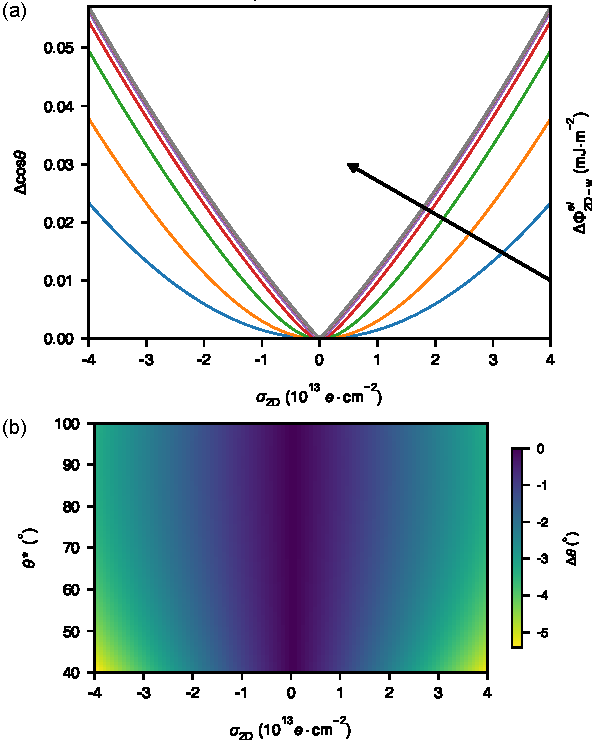
\includegraphics[width=0.85\linewidth]{../img/2d-ph-dependency.pdf}
\caption{\label{fig:Delta-cos-dependency}
(a) \(\Delta\cos\theta\) as a function of \(\sigma_{\mathrm{2D}}\).The concentration varies from \(10^{0}\) to \(10^{-7}\) mol\(\cdot\mathrm{L}^{-1}\) (b) \(\Delta\theta\) as a function of \(\sigma_{\mathrm{2D}}\) and the hypothetical contact angle on a charge-neutral 2D material layer \(\theta^{*}\). c\(_{\text{0}}\) is taken as \(10^{-7}\) mol\(\cdot\mathrm{L}^{-1}\).}
\end{figure}

Consider that the aqueous phase contains a 1:1 electrolyte with
concentration \(c_{0}\), the thickness of the Helmholtz plane
\(d_{\mathrm{H}}=3\ \mathrm{\AA}\) \cite{mcclendon_thickness_1927}, and
the surface tension of water \(\gamma_{\mathrm{w}}=72.8\) mJ\(\cdot
\mathrm{m}^{-2}\) at \(T=298\) K, we calculate the magnitude of
\(\Delta\Phi_{\mathrm{2D-w}}^{el}\) and \(\Delta\cos\theta\) as function
of \(\sigma_{\mathrm{2D}}\), as shown in
Fig. \ref{fig:Delta-cos-dependency}(a). We discover that both the
changes in the magnitude of interfacial adhesion energy and the
contact angle become more pronounced when the concentration of
electrolyte is lower. On the contrary, in conventional electrowetting
model, \(\Delta\theta\) is governed by the constant capacitance of the
dielectric layer and is almost irrelevant to the \(c_{0}\). The results indicate that the variation of \(c_{0}\) has a significant impact on \(\Delta
\Phi_{\mathrm{2D-w}}^{el}\) and \(\Delta \cos \theta\) in the
electrowetting on doped 2D materials. This is due to the fact that the
interfacial potential \(\psi_{\mathrm{2D}}\) is affected by both the
surface charge \(\sigma_{\mathrm{2D}}\) and \(c_{0}\), as indicated by
Eq. (\ref{eqn:psi-L}) and (\ref{eqn:psi-2D}). When \(c_{0}\) is lower, a
larger potential is required to be built upon the interface, giving
rise to a larger change in the interfacial wetting property.

Although the ``real'' contact angle of a 2D material can be tedious to
determine, it is still possible to estimate the magnitude of contact
angle change due to the electrowetting effect, by assuming that the
hypothetical contact angle \(\theta^{*}\) on a charge-neutral 2D
material layer. \(\theta^{*}\) consists of the effect of intrinsic
wettability, surface contamination as well the wetting translucency of
the 2D material-liquid interface. Fig. \ref{fig:Delta-cos-dependency}(b)
shows the magnitude of contact angle decrease as a function of both
\(\sigma_{\mathrm{2D}}\) and \(\theta^{*}\), when \(c_{0}=10^{-7}\)
mol\(\cdot \mathrm{L}^{-1}\) (e.g. ideally pure water). Within the range
of typical contact angles reported on graphene (ca. 40\(^{\circ}\) \textasciitilde{}
100\(^{\circ}\)), and a doping level of \(-5\times10^{13}\) \textasciitilde{}
\(5\times10^{13}\) \(e \cdot \mathrm{cm}^{-2}\), we find that the maximum
magnitude \(\Delta\theta\) is only ca. 7\(^{\circ}\) when doping level is
as high as \(\pm 5 \times 10^{13}\) \(e\cdot \mathrm{cm}^{-2}\),
essentially smaller than previously reported values which were
measured both under smaller doping levels
\cite{hong_mechanism_2016,ashraf_doping-induced_2016}.  Due to the
saturation of CO\(_{\text{2}}\) in water and soluble contaminants, the effect of
electrowetting may be even less prominent in real
situations. Therefore we believe that the electrowetting effect theory
on 2D materials alone, cannot explain the current findings of
doping-induced wettability change on graphene.


Practically in a contact angle measurement, the amount of water varies
from pL (using environmental scanning electron microscopy, ESEM) to
\(\mathrm{\mu L}\) (using goniometer). Unlike nanodroplet models used in
MD contact angle simulations, the droplets used experimentally are
large enough to be exposed to both pristine and defect 2D surface, and
can therefore be trapped in the local minimal state caused by nanoscale
defects \cite{raj_wettability_2013}, giving rise to uncertainty of the
measured contact angle. Meanwhile, it is widely observed that
nanopores and macroscopic cracks exist in the transferred 2D material,
increasing the adhesion interaction between the substrate and the
water droplet.

\begin{figure}[htbp]
\centering
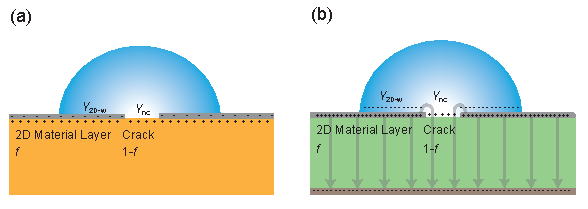
\includegraphics[width=0.95\linewidth]{../img/scheme-crack.pdf}
\caption{\label{fig:scheme-crack}
Schematic drawing of the incomplete surface coverage in (a) substrate doping and (b) electrostatic doping systems. In both cases the aqueous phase is exposed directly to the substrate, leading to a discrepancy of apparent wetting properties compared with theoretical values.}
\end{figure}

We further consider the cases where the 2D material does not
completely cover the substrate. In both the substrate-induced doping
(see Fig. \ref{fig:scheme-crack}(a)) and the electrostatic doping (see
Fig. \ref{fig:scheme-crack}(b)) systems, substrate surface charge still
exists in non-covered regions: in surface doping the charged dopants
(i.e. polyelectrolytes) will instantly build up a EDL near the
substrate surface, while in electrostatic doping the electric
displacement field still forms between the conducting 2D material and
the gate electrode via the non-covered region, also causing the ions
to accumulate at the substrate-water interface. The interfacial
adsorption density of ions can essentially be larger than the surface
charge density on 2D material, due to the partial screening of
electric displacement field of the 2D material
\cite{tian_multiscale_2016,Shih2015PartiallyScreened,Muruganathan_2015,Huttmann_2015}. Since
the electrowetting effect is amphipolar, the accumulation of cations
and anions at the 2D material surface or the non-covered region
both contribute to the decrease of the apparent surface tension
\(\hat{\gamma}_{\mathrm{2D-w}}\). We assume that the electrowetting at
the non-covered region is described by the classical Young-Lippman
\(\Delta
\gamma_{\mathrm{nc}}=-\frac{\sigma_{\mathrm{2D}}^{2}}{2C_{\mathrm{nc}}}\),
where \(C_{\mathrm{nc}}\) is the effective capacitance of the
non-covered region (taken as the EDL capacitance in substrate doping,
or the geometric capacitance of dielectric layer in electrostatic
doping). We therefore describe \(\Delta
\hat{\gamma}_{\mathrm{2D-w}}\) as a combined effect of the
electrowetting on both pristine 2D material surface and non-covered substrate surface,
characterized by the surface coverage index \(f\):
\begin{equation}
\label{eqn:apparent-gamma-combined}
\begin{aligned}
\Delta \hat{\gamma}_{\mathrm{2D-w}} &= f \Delta \gamma_{\mathrm{2D-w}} + (1-f)\Delta \gamma_{\mathrm{nc}} \\
&= f \Delta \gamma_{\mathrm{2D-w}}  -\frac{1}{2}(1-f)\frac{\sigma_{\mathrm{2D}}^{2}}{C_{\mathrm{nc}}}
\end{aligned}
\end{equation}

It should also be noted that in electrowetting experiments
where additional charge is doped to the 2D material via dielectric
layer \cite{hong_mechanism_2016}, the initial doping density
\(\sigma_{\mathrm{i}}\) should also be considered to explain the
asymmetric electrowetting behavior. In an electrowetting system where a
dielectric layer with geometric capacitance \(C_{\mathrm{d}}\) and external
voltage \(V_{\mathrm{2D}}\) is applied to the 2D material, the doping
density in the 2D material is calculated as \cite{tian_multiscale_2016}:
\begin{equation}
\label{eqn:doping-vm-2D}
V_{\mathrm{2D}} = \frac{\sigma_{\mathrm{2D}} - \sigma_{\mathrm{i}}} {C_{\mathrm{d}}} 
                 + \int_{\sigma_{\mathrm{i}}}^{\sigma_{\mathrm{2D}}} 
                   \frac{1}{C_{\mathrm{2D}}} \mathrm{d}\sigma'
\end{equation}
where \(C_{\mathrm{2D}}\) is the quantum capacitance of the 2D material, which is proportional to the density of states (DOS) \(g(E)\) at energy level \(E\): \(C_{\mathrm{2D}}=g(E)e^{2}\).

\begin{figure}[htbp]
\centering
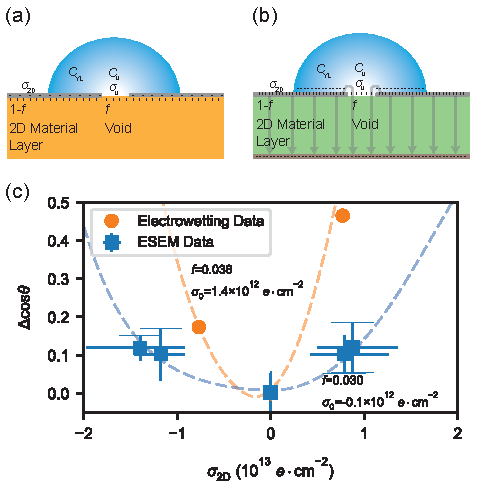
\includegraphics[width=0.95\linewidth]{../img/plot-fitting.pdf}
\caption{\label{fig:f-nc-exp}
Theoretical and fitted experimental data of \(\Delta\cos\theta\) as a function of \(\sigma_{\mathrm{2D}}\). The electrowetting data are extracted from Ref. \cite{hong_mechanism_2016}; the ESEM data are extracted from Ref. \cite{ashraf_doping-induced_2016}.}
\end{figure}

To examine the effect of incomplete 2D material coverage, we select
two sets of reported experimental measurements of the wettability on
doped graphene sheet, namely the contact angles of substrate-doped
graphene measured by ESEM from Ref. \cite{ashraf_doping-induced_2016}
and the contact angles of electostatically-doped graphene via
goniometer from Ref. \cite{hong_mechanism_2016}. The contact angle at
experimentally ``charge-neutral'' condition (graphene attached to SiO\(_{\text{2}}\)
substrate for ESEM experiment or \(V_{\mathrm{2D}}=0\) V in
electrowetting experiment, however \(\sigma_{\mathrm{2D}}\) may not be 0
due to existence of \(\sigma_{\mathrm{i}}\)) is used as reference for
calculating \(\mathrm{d}\cos\theta\). We use
Eq. \ref{eqn:apparent-gamma-combined} to extract \(f\) and
\(\sigma_{\mathrm{i}}\) for both experiments, as seen in
Fig. \ref{fig:f-nc-exp}. We observe that in both experimental data sets,
the measured \(\Delta \cos \theta\) is essential larger than the
theoretical value derived from the Gouy-Chapman-Stern model described
here. Fitting results reveals both systems are lightly p-doped in the
``charge-neutral'' condition, which corresponds well with other
experimental reports
\cite{Shih2015PartiallyScreened,goniszewski_correlation_2016}.  The
fitted \(f\) values for both systems are as small as 3.7\%-3.8\%,
indicating the graphene layers are mostly complete. It is very
surprising to find out that due to large discrepancy of wetting
behavior on the 2D material and the underlying substrate, the measured
contact angle change can be greatly influenced by the existence of
minor defects in the 2D material. Our calculations show that extreme
care should be taken to interpret the true doping-tunable wetting
behavior of 2D materials.


The doping-induced tuning of wetting on 2D materials opens a novel
avenue for 2D-material-based liquid manipulating devices. Unlike
conventional electrowetting on dielectric (EWOD) setup, no counter
electrode is required in the liquid phase, ensuring simpler device
design. Although Eq. \ref{eqn:Delta-Phi-exact} shows that the
electrowetting effect of 2D material is only dependent on the surface
charge \(\sigma_{\mathrm{2D}}\), practically it is more favorable to
achieve the desired electrowetting by applying a smaller
\(V_{\mathrm{2D}}\). A usual setup for electrostatic doping of 2D
material involves the use of high-k dielectric or ionic gating
\cite{Das_2008,Radisavljevic_2011,Xu_2011,Newaz_2012}, where the
\(C_{\mathrm{d}}\) is comparable with \(C_{\mathrm{2D}}\). Therefore the
contribution of \(C_{\mathrm{2D}}\) in Eq. \ref{eqn:doping-vm-2D} cannot
be ignored. Combing Eqs. \ref{eqn:psi-L}, \ref{eqn:psi-2D} and
\ref{eqn:doping-vm-2D}, we get:

\begin{align}
\label{eqn:dV-sigma-2D}
\mathrm{d} V_{\mathrm{2D}} &= \left(\frac{1}{C_{\mathrm{d}}} +
\frac{1}{C_{\mathrm{2D}}}\right) \mathrm{d}\sigma_{\mathrm{2D}} \\
\label{eqn:dpsi-sigma-L}
\mathrm{d} \psi_{\mathrm{2D}} &= -\left( \frac{1}{C_{\mathrm{H}}}
+ \frac{1}{C_{\mathrm{L}}} \right) \mathrm{d}\sigma_{\mathrm{L}}
\end{align}
and by substituting \(\sigma_{\mathrm{2D}} = -\sigma_{\mathrm{L}}\), we derive the ratio between \(\psi_{\mathrm{2D}}\) and \(V_{\mathrm{2D}}\), named as \(\beta\):
\begin{equation}
\label{eqn:beta}
\beta = \frac{\mathrm{d} \psi_{\mathrm{2D}}}{\mathrm{d}
V_{\mathrm{2D}}} = \dfrac{\dfrac{1}{C_{\mathrm{L}}} +
\dfrac{1}{C_{\mathrm{H}}}}{\dfrac{1}{C_{\mathrm{d}}} + \dfrac{1}{C_{\mathrm{2D}}}}
\end{equation}
at a certain \(c_{0}\), the larger \(\beta\) is, the higher tunability in
wettability of the 2D material will be. On the device side, it can be
achieved if both \(C_{\mathrm{d}}\) and \(C_{\mathrm{2D}}\) are
larger. Increasing the value of \(C_{\mathrm{2D}}\) can be implemented
by replacing graphene--a 2D semimetal, with a 2D semiconductor, such
as TMDC \cite{tian_multiscale_2016}. Here we evaluate a
2D-material-based electrowetting device consists of a 2 nm thick HfO\(_{\text{2}}\)
dielectric layer with \(\epsilon_{\mathrm{d}}=24.0\), and an 2D material sheet
selected from graphene, silicene (2D allotrope of Si), germanene (2D
allotrope of Ge), MoS\(_{\text{2}}\), MoTe\(_{\text{2}}\), WS\(_{\text{2}}\) and WTe\(_{\text{2}}\) (see
Fig. \ref{fig:dcos-all-2D}(a)). The DOS and \(C_{\mathrm{2D}}\) are
calculated from first-principle simulations using HSE06 hydrid
functional (see Ref. \cite{tian_multiscale_2016}). The magnitude of \(\Delta \cos \theta\) as a function of \(V_{\mathrm{2D}}\) in devices based on different 2D materials is shown in Fig. \ref{fig:dcos-all-2D}(b).
\begin{figure}[htbp]
\centering
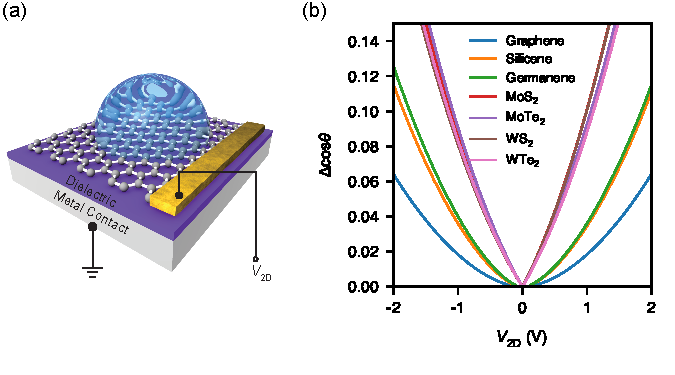
\includegraphics[width=0.95\linewidth]{../img/dcos-all-2D.pdf}
\caption{\label{fig:dcos-all-2D}
(a) Schematic illustration of the 2D-material-based electrowetting device. (b) \(\Delta\cos\theta\) as a function of \(V_{\mathrm{2D}}\) for selected 2D materials.}
\end{figure}

As expected in Eq. \ref{eqn:beta}, at the same \(V_{\mathrm{2D}}\) level,
the 2D TMDC semiconductors (MoS\(_{\text{2}}\), MoTe\(_{\text{2}}\), WS\(_{\text{2}}\), WTe\(_{\text{2}}\)) exhibit a much
higher response \(\Delta \cos \theta\) than 2D semimetals (silicene,
germanene and graphene). We can briefly rank the voltage tunability of
the selected 2D materials by their DOS: MoTe\(_{\text{2}}\) > MoS\(_{\text{2}}\) > WTe\(_{\text{2}}\) > WS\(_{\text{2}}\)
> germanene > silicene > graphene. Notably, TMDCs can achieve a
\(\Delta \Phi_{\mathrm{2D}}\) as high as 0.15 when
\(V_{\mathrm{2D}}=\pm1.5\) V is applied, corresponding a contact angle
decrease at the magnitude of 10\(^{\circ}\) when the intrinsic contact
angle is ca. 90\(^{\circ}\).  A high-DOS 2D material further suppresses
electrochemical reactions at the solid-liquid interface, as less
electrochemical potential (i.e. the Fermi level \(E_{\mathrm{F}}\)) is
required. We conclude that a 2D material with higher DOS can
essentially reduced the voltage needed for doping, pushing
liquid-phase 2D-material-based devices to a more operational regime.


In conclusion, we propose a multiscale approach for modeling the
doping-induced tunable wettability of 2D materials, by combining the
reorientation effect of water molecules estimated by MD simulations,
and the electrowetting effect calculated by a continuum model. Taking
graphene as an example, we find that electrostatic interaction plays a
major role at both scales for the graphene-water interface. We further
show that, by considering the incomplete coverage of 2D material on
the substrate, it is possible to evaluate the recent findings of
doping-induced tuning of graphene's wettability with the proposed
model. We find that minor surface incompleteness can cause great
discrepancy in the measured value of interfacial wettability, and
extreme care should be taken to interpret the observed
electrowetting phenomena. In addition, we prove that a 2D material
with higher density of states can essentially reduce the gating
voltage in a 2D-material-based electrowetting device, and rank the
tunability of the 2D materials as: MoTe\(_{\text{2}}\) > MoS\(_{\text{2}}\) > WTe\(_{\text{2}}\) > WS\(_{\text{2}}\) >
germanene > silicene > graphene. Our multiscale analysis provides a
comprehensive view of the wettability of 2D material interface, and we
believe operational 2D-material-based liquid manipulating devices will
be facilitated by the principles presented in this letter.
\bibliography{ref}
\end{document}